\documentclass{beamer}
\usepackage{beamerthemesplit}
\usepackage{wrapfig}
\usetheme{SPbGU}
\usepackage{pdfpages}
\usepackage{amsmath}
\usepackage{cmap} 
\usepackage[T2A]{fontenc} 
\usepackage[utf8]{inputenc}
\usepackage[english,russian]{babel}
\usepackage{indentfirst}
\usepackage{amsmath}
\usepackage{tikz}
\usepackage{multirow}
\usepackage[noend]{algpseudocode}
\usepackage{algorithm}
\usepackage{algorithmicx}
\usetikzlibrary{shapes,arrows}
\usepackage{fancyvrb}
\usepackage{tikz}
\usepackage{pgfplots}
\usepackage{sidecap}
\pgfplotsset{compat=1.9}
\newtheorem{rutheorem}{Теорема}
\newtheorem{ruproof}{Доказательство}
\newtheorem{rudefinition}{Определение}
\newtheorem{rulemma}{Лемма}

\title[]{Зачем биологам синтаксический анализ}
% То, что в квадратных скобках, отображается в левом нижнем углу. 
\institute[СПбГУ]{
    Санкт-Петербургский государственный университет \\
    Лаборатория языковых инструментов JetBrains}

% То, что в квадратных скобках, отображается в левом нижнем углу.
\author[Артём Горохов]{Артём Горохов}
\date{15 октября 2016г.}

\begin{document}
    
    \definecolor{red}{RGB}{255,0,0}
    
    \begin{frame}
        \begin{center}
            {
\includegraphics[width=1.5cm]{pictures/SPbGU_Logo.png}}
        \end{center}
        \titlepage
    \end{frame}
    
    \begin{frame}
    	\frametitle{Биоинформатика}
    	\begin{itemize}
		    \item Множество задач, всязанных с обработкой и понимаением биологических данных
    		\item Одна из задач - поиск организмов в метагеномных сборках
    	\end{itemize}
    \end{frame}

    \begin{frame}
        \frametitle{Геном}
        \begin{itemize}
            \item Геном (последовательность ДНК) - длинная последовательность нуклеотидов
            \item На деле строка в алфавите \{A, C, G, T\}
        \end{itemize}
    \end{frame}

    \begin{frame}
        \frametitle{Секвенирование}
        \begin{itemize}
            \item Из биологического материала получаются риды - последовательности строчек в алфавите \{A, C, G, T\}
            \item Риды склеиваются в более длинные строки - контиги
            \item Множество полученных контигов – сборка
        \end{itemize}
    \end{frame}

    \begin{frame}
        \frametitle{Сборки}
        В зависимости от биологического материала, из которого получаются данные, сборки
        бывают:
        \begin{itemize}
            \item single-cell. Cборки, для получения которой была взята одна или несколько
            (до четырёх) клеток колонии
            \item multi-cell. В качестве биологического материала были взяты тысячи или даже десятки тысяч клеток одного штамма
            \item метагеномные. Данные взяты из среды обитания целевой колонии, в которой были как её представители, так и соседствующих
        \end{itemize}
    \end{frame}

    \begin{frame}
        \frametitle{Геном}
        Процесс расшифровки генома:
        \begin{itemize}
            \item секвенирование
            \item ассемблирование
            \item финишинг
        \end{itemize}
    \end{frame}
    
    \begin{frame}
        \frametitle{Геном}
        Процесс расшифровки генома:
        \begin{itemize}
            \item секвенирование
            \item ассемблирование
            \item финишинг
        \end{itemize}
    \end{frame}


    
    \begin{frame}
        \frametitle{Метагеномная сборка}
        \begin{itemize}
            \item Есть множество цепочек, подлежащих анализу
            \item Все объединяются в граф
        \end{itemize}
        
        \begin{figure}[t]
            \begin{align*}
                CUUCA {\color{red} GAC} &{\color{red} UCCGACU}  UCG \\
                                        &{\color{red} UCCGACU} CGUUU \\
                GCAUU {\color{red} GAC} &{\color{red} UC}
            \end{align*}
        \end{figure}
        
        \begin{figure}[b]
            \centering
            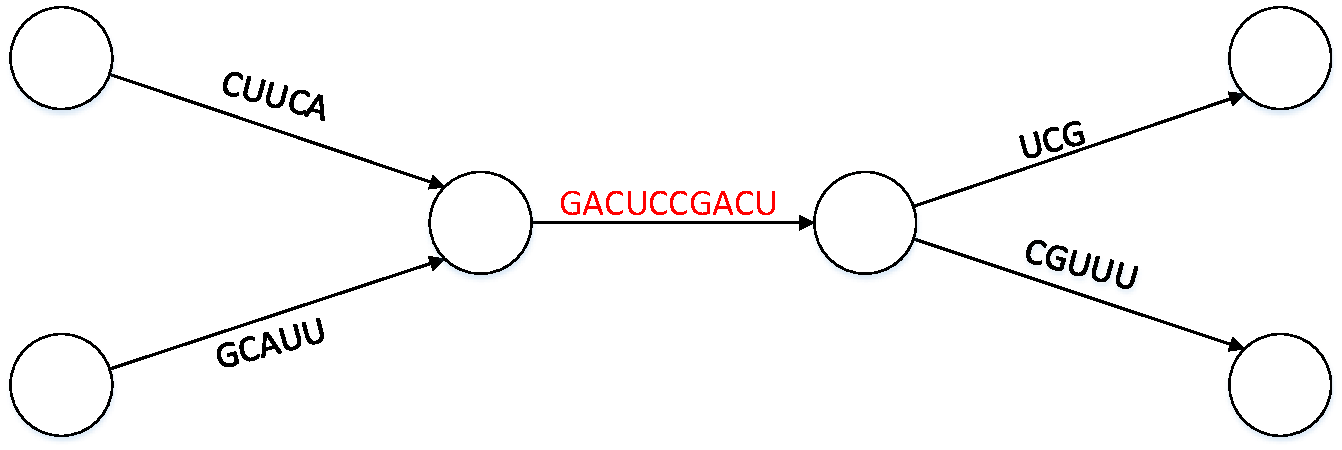
\includegraphics[width=8cm]{pictures/methagenEx.pdf}  
        \end{figure}
          
        
    \end{frame}

    \begin{frame}
    \frametitle{Структура цепочек}
    \begin{tabular}{p{6cm} p{5cm}}
        \begin{itemize}
            \item КС грамматика может описать вторичную структуру
        \end{itemize}
        \\
        \\
        \\
        $$
        GGAAGAUCG...GCA...  =>
        $$
        &
        \multirow{-10}*{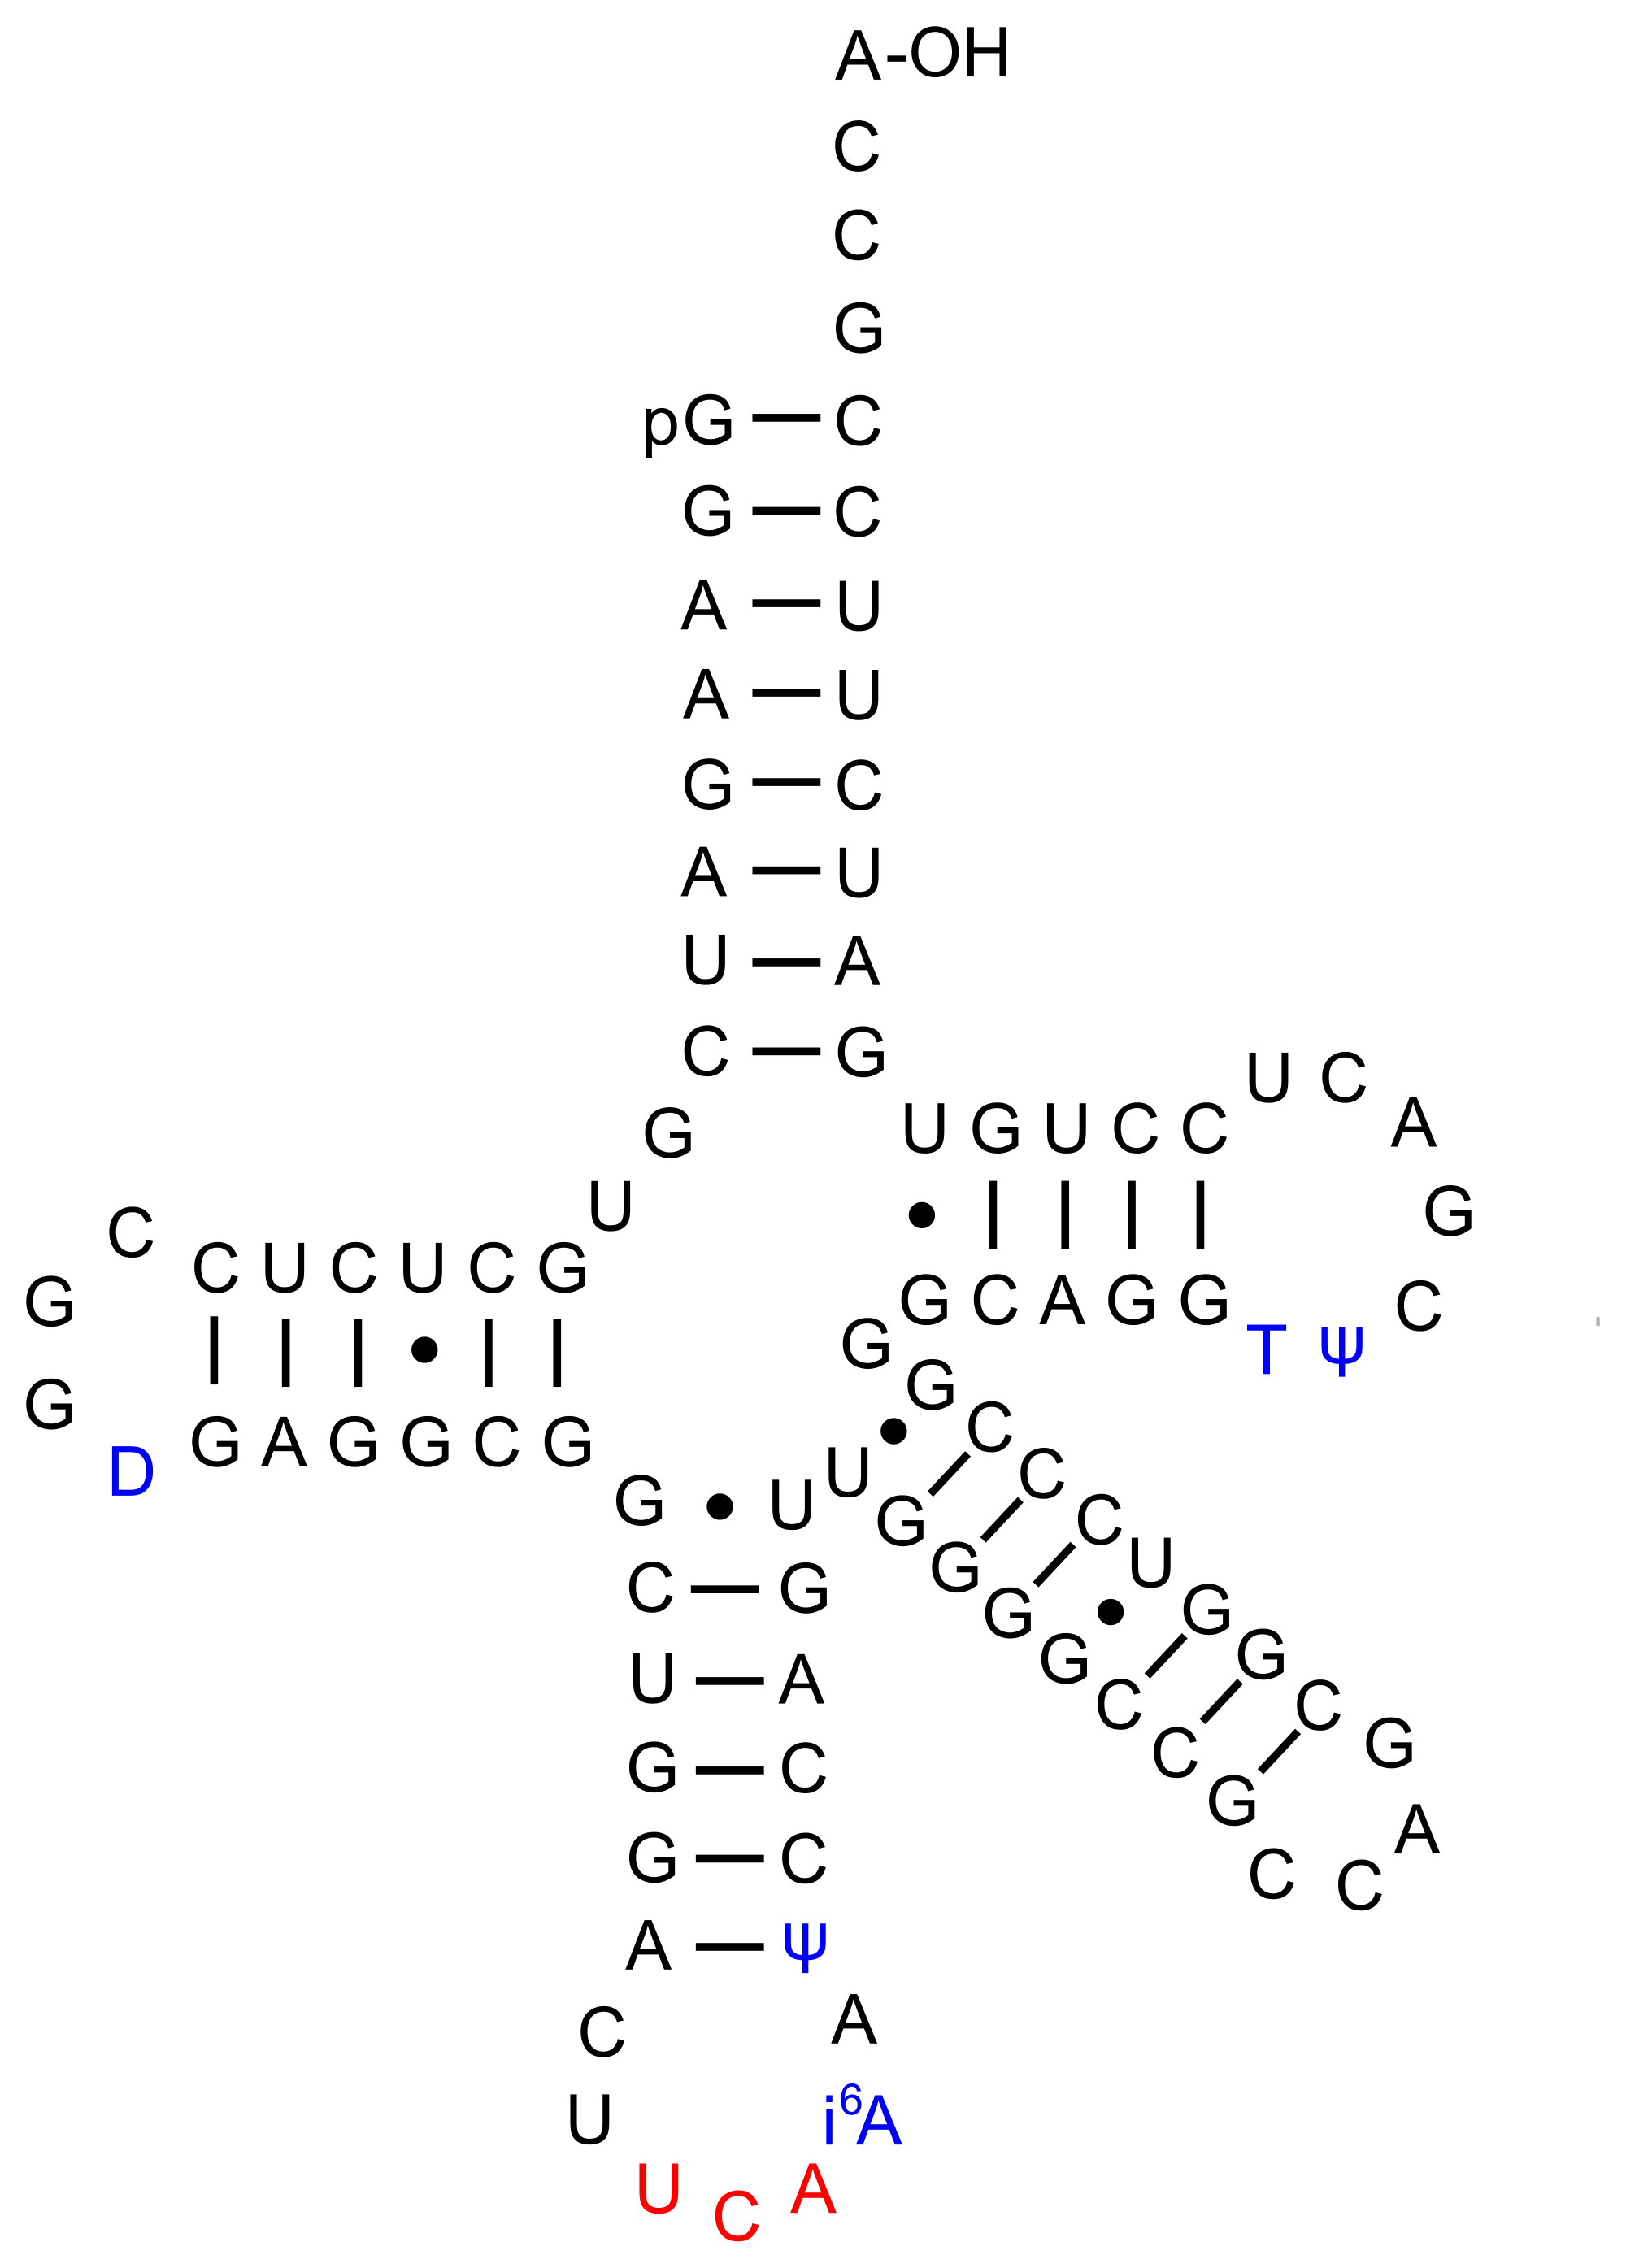
\includegraphics[width=5.2cm]{pictures/TRNA.png}}
    \end{tabular}  
    
    \end{frame}
    
    \begin{frame}
        %\frametitle{Вторичная структура 16s}
        \begin{figure}[t]
            \centering
            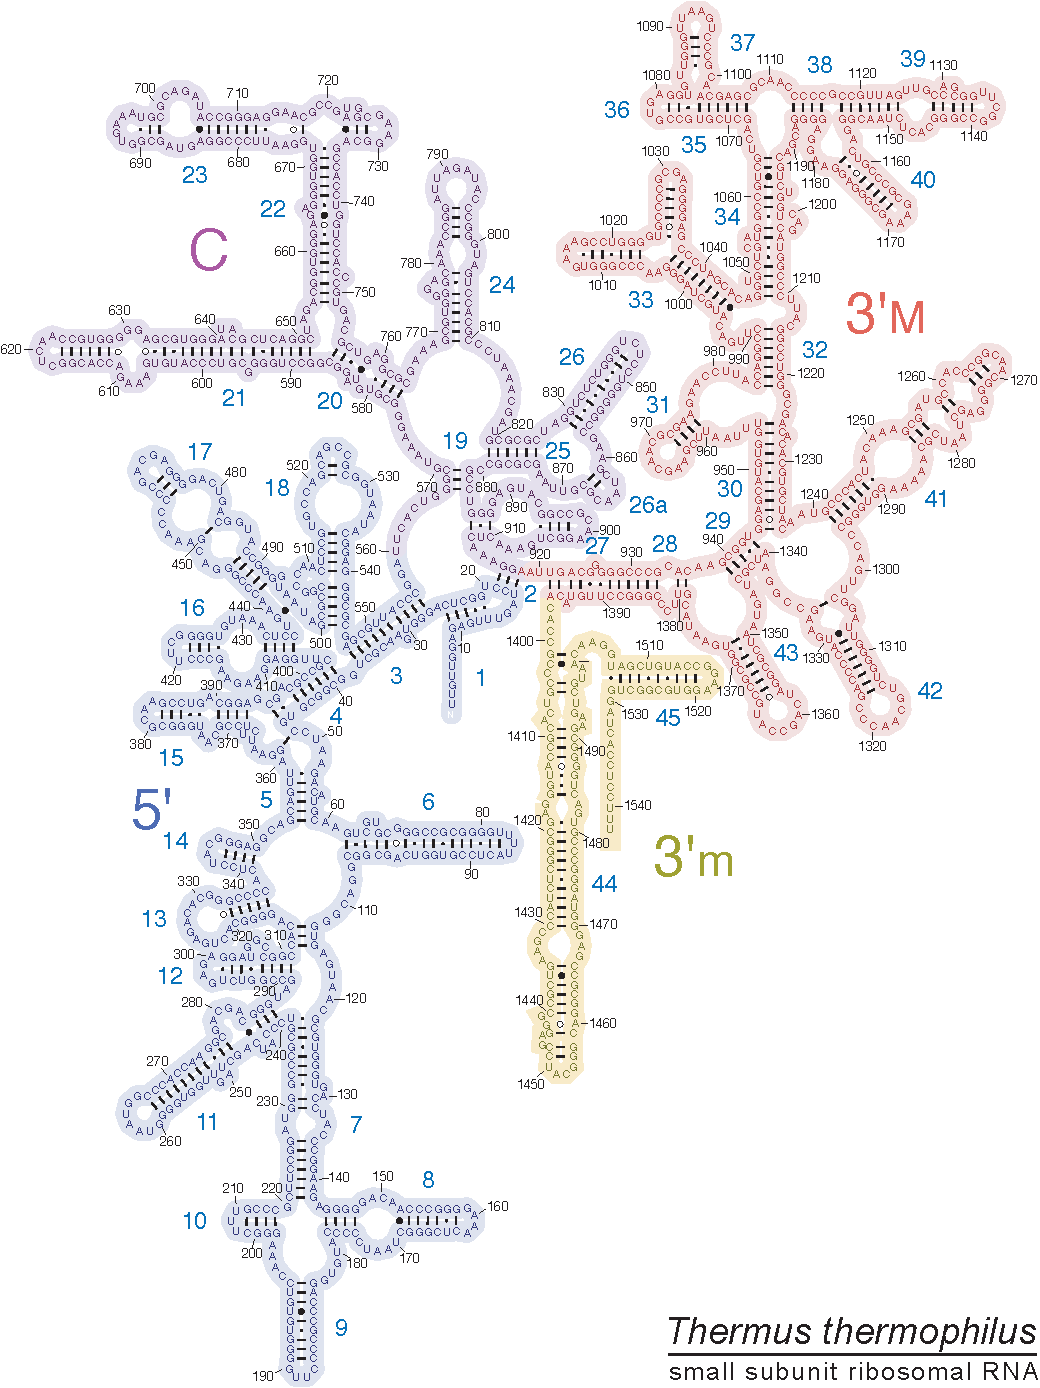
\includegraphics[width=6.7cm]{pictures/thermus_16s_2ndry.pdf}
        \end{figure}
    \end{frame}

    \begin{frame}
		\frametitle{GLL}
		\begin{itemize}
			\item Generalized LL
			\item Нисходящий синтаксический анализатор
			\item В лучшем случае работает за линейное время, в худшем - за $O(n^{3})$
			\item Строит все возможные выводы цепочки
		\end{itemize}
	\end{frame}
	
	\begin{frame}
		\frametitle{GLL}
		\begin{figure}[t]
			\begin{tabular}{p{3cm} p{3cm} p{3cm}}
				Вход: a a b
				&
				\multirow{1}*{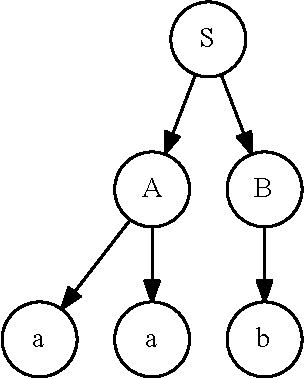
\includegraphics[width=3cm]{pictures/GLLtree0.pdf}}
				&
				\multirow{1}*{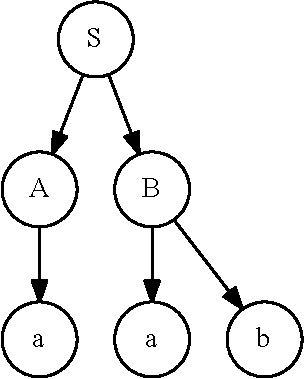
\includegraphics[width=3cm]{pictures/GLLtree1.pdf}}
				\\ & & \\
				Грамматика:& & \\
				{$\begin{aligned}
					S\ =&\ A\ B \\
					A\ =&\ a\ a \\
					|&\ a \\
					B\ =&\ b \\
					|&\ a\ b
					\end{aligned}$} & &
			\end{tabular}
			
		\end{figure}
	\end{frame}
	
	\begin{frame}
		\frametitle{GLL для графов}
		\begin{tabular}{p{7cm} p{5cm}}
			\begin{itemize}
				\item На вход поступает граф, задающий все входные цепочки
				\item На рёбрах терминалы
			\end{itemize}
			&
			% Картинка
			\multirow{-4}*{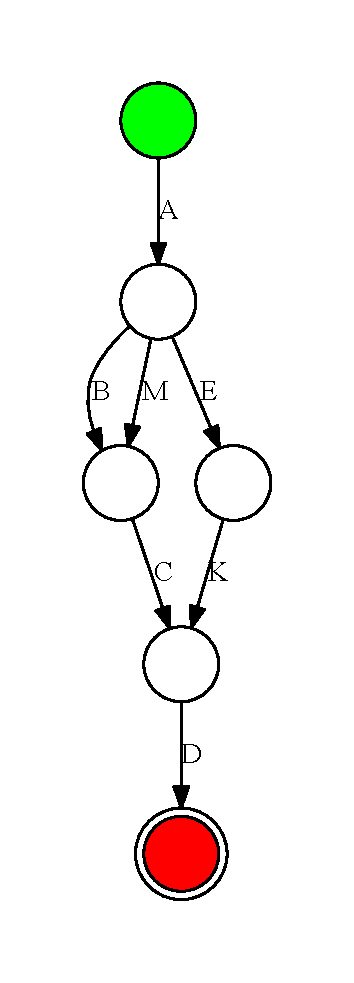
\includegraphics[width=3cm]{pictures/graphGLLexample.pdf}}
			\\ &
			\\ &
			\\ 
			$$
			\{A B C D;
			A M C D;
			A E K D \} =>
			$$ &
		\end{tabular}
	\end{frame}

    \begin{frame}
        \frametitle{Увеличение производительности}
        \begin{itemize}
            \item Полученные метагеномные сборки не поддаются анализу без предварительных преобразований
            \item Сам алгоритм нуждается в модернизации
        \end{itemize}
    \end{frame}

    \begin{frame}
        \frametitle{Фильтрация рёбер}
        \begin{itemize}
            \item Infernal позволяет распознавать структуры в линейном входе
            \item Рёбра, длиннее искомых структур можно делить на части и проверять infernal'ом
        \end{itemize}
    \end{frame}

    \begin{frame}
        \frametitle{Разбиение на компоненты}
        \begin{itemize}
            \item После фильтрации рёбер граф распадается на компоненты связности
            \item Можно запускать анализатор независимо на разных компонентах
        \end{itemize}
    \end{frame}
    
    \begin{frame}
        \frametitle{Отказ от построения дерева}
        \begin{itemize}
            \item Парсер возвращает лишь границы и длину найденой цепочки
            \item Восстановление цепочки идёт путём извлечения подграфа
            \item Ложные фильтруются infernal
        \end{itemize}
        
        \begin{figure}[b]
            \centering
            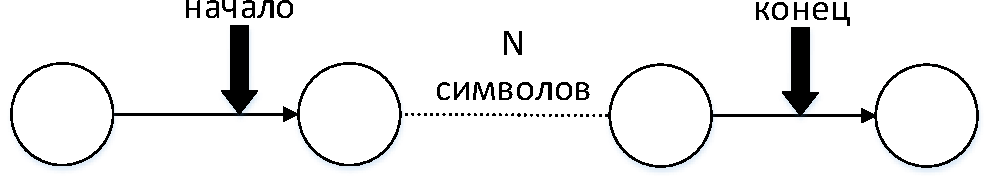
\includegraphics[width=8cm]{pictures/noTree.pdf}  
        \end{figure}
    \end{frame}

    \begin{frame}
        \frametitle{Преобразование грамматики к автомату}
        \begin{tabular}{p{5cm} p{4cm}}
            Грамматика
            \begin{figure}[t]
                {$\!\begin{aligned}
                    S\ =&\ A\ A\ A\ A\ A \\
                       |&\ A\ a\ A\ A\ A \\
                    A\ =&\ S\ A \\
                       |&\ a\ A \\
                       |&\ a
                    \end{aligned}$}
            \end{figure}
            &
            Автомат
            \begin{figure}[t]
                \centering
                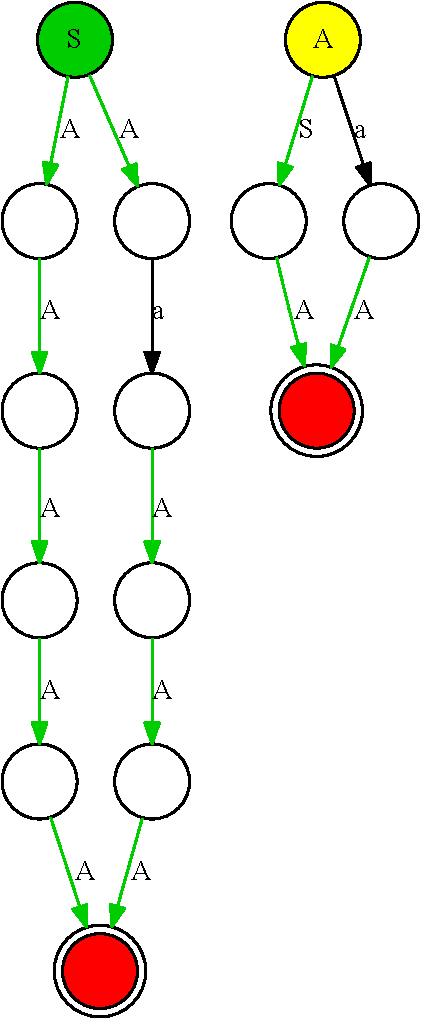
\includegraphics[height=7cm]{pictures/initialNFA.pdf}
            \end{figure}
        \end{tabular}
    \end{frame}

\begin{frame}
    \frametitle{Минимизация автомата}
    \begin{tabular}{p{5cm} p{5.5cm}}
        Изначальный автомат
        \begin{figure}[t]
            \centering
            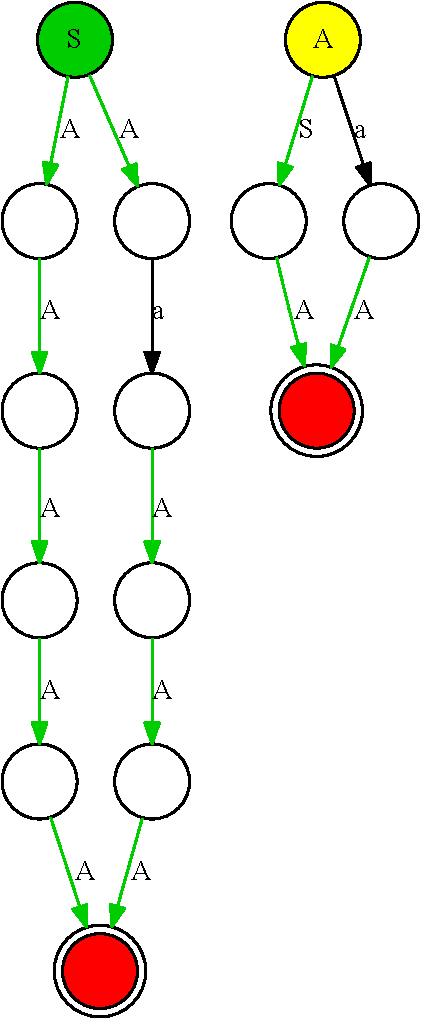
\includegraphics[height=7cm]{pictures/initialNFA.pdf}
        \end{figure}
        &
        Минимизированый автомат
        \begin{figure}[t]
            \centering
            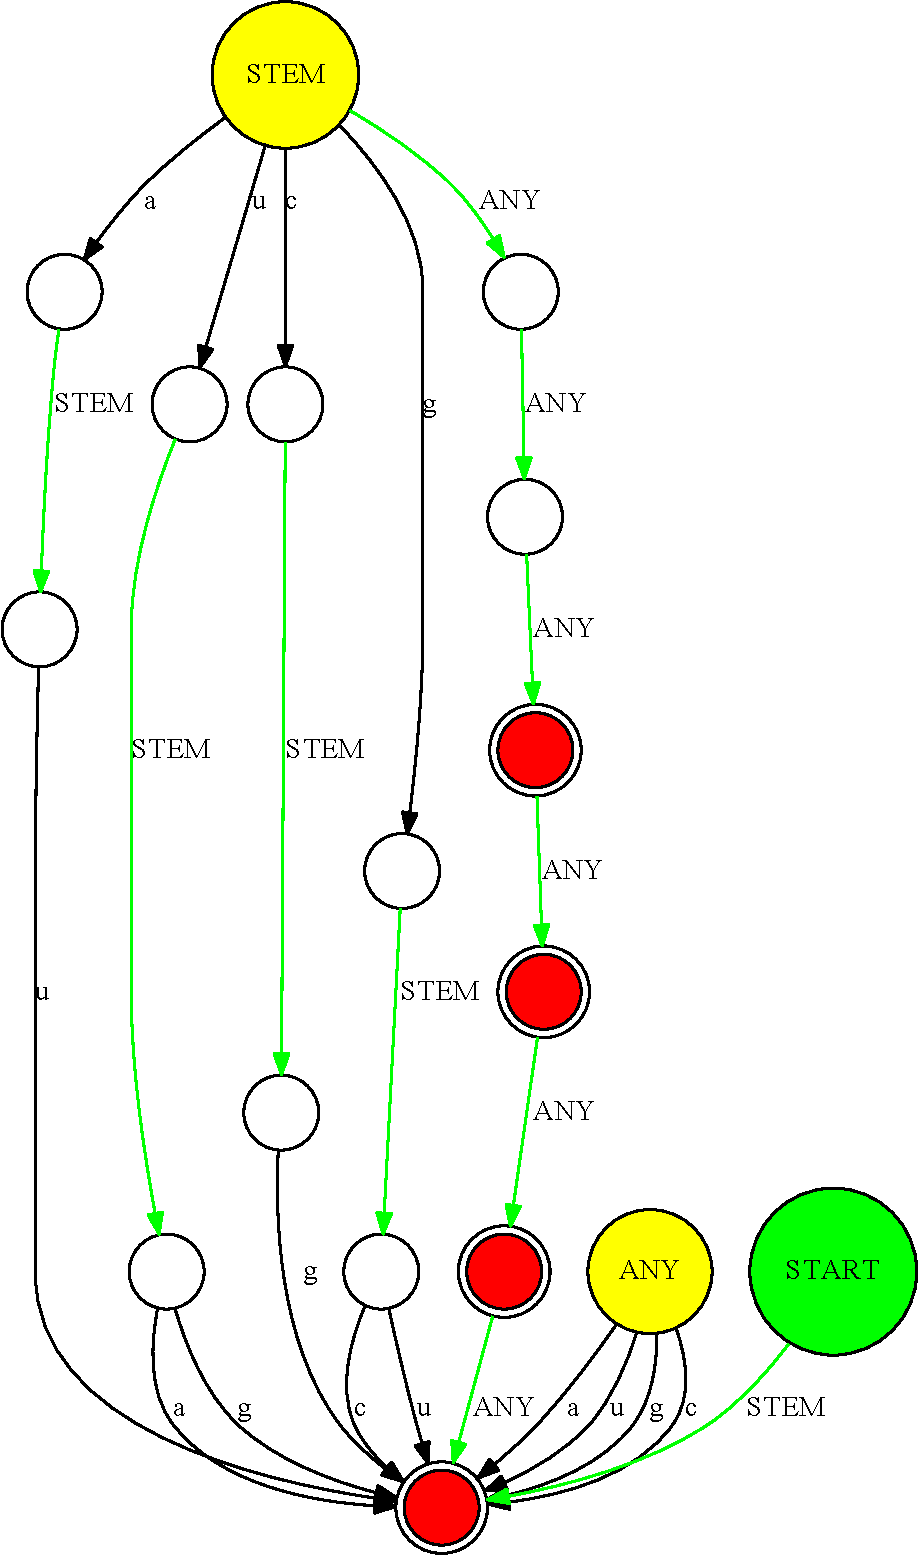
\includegraphics[height=7cm]{pictures/minimizedDFA.pdf}
        \end{figure}
    \end{tabular}
\end{frame}

\begin{frame}
    \frametitle{Эксперименты}
    \begin{tabular}{| p{2.5cm} | p{2cm} | p{2.5cm} |}
        \hline
                     & начальная грамматика & мин. автомат \\ \hline
        Время работы & 10 часов             & 3ч. 40 мин. \\ \hline
    \end{tabular}
\end{frame}

\begin{frame}
    \frametitle{Направление работ}
    \begin{itemize}
        \item Детальный анализ качества результата
        \item Возможно, можно сильнее фильтровать граф, применяя infernal
        \item Поиск полноразмерных 16s
        \item Поиск других структур
    \end{itemize}
\end{frame}


\end{document}
